\documentclass[../main.tex]{subfiles}
\begin{document}

\subsection{Experimento 1}
\begin{enumerate}
    \item Pasaremos a traer los materiales a la mesa de trabajo.
    \item Marcaremos cada pesa ($m_1$, $m_2$, $m_3$, $m_4$) para diferenciarlas, 
    luego pasaremos a pesar las masas en la balanza digital y medir la 
    longitud natural del resorte en la barra transversal, una vez realizado esto pasaremos a anotar en una hoja de calculo los masas y longitud obtenidas.
    \item Nivelaremos la barra transversal y el soporte universal.
    \item Realizaremos cinco combinaciones de masas ($m_3$, $m_1+m_3$, $m_3+m_2$, $m_3+m_4$, $m_1+m_2+m_3$) 
    donde cada combinación será enganchada al extremo del resorte y el otro extremo del resorte estará enganchado 
    a la barra transversal del soporte universal.
    \item Un compañero sostendrá el soporte universal, otro compañero enganchara una combinación de masas para 
    pasar a medir con una regla la longitud que tendrá ahora el resorte al ser enganchado por una combinación de 
    estas masas, estos valores de longitud serán anotados en la hoja de cálculos con su respectiva incertidumbre.
    \item Este procedimiento de enganchar la masa al resorte y medir la longitud que tendrá el resorte 
    ahora será realizado para las cinco combinaciones de masas.
    \item Esto nos permitirá determinar la constante del resorte de la 
    gráfica F vs X realizando ajustes de mínimo cuadrados.
\end{enumerate}
\subsection{Experimento 2}
\begin{enumerate}
    \item En este caso pondremos el soporte universal al extremo 
    de la mesa de trabajo apoyada de la pared, la razón será por 
    que al poner las combinaciones de masas al resorte y este 
    empiece a oscilar no queremos que las masas choquen con la mesa 
    impidiendo la medición.
    \item Un compañero tendrá un cronómetro en la mano, otro 
    compañero sostendrá el soporte universal y otro compañero soltará 
    una combinación de masas el cual esta enganchado al resorte, 
    se soltara con mucho cuidado evitando que el resorte se mueva a 
    sus extremos, al realizar esto nos damos cuenta que no tiene 
    estabilidad el resorte ya que  mueve mucho así que el grupo 
    decidió poner una cinta alrededor del extremos que tiene el 
    resorte y la barra transversal para darle más estabilidad.
    \item Soltaremos una combinación de 
    masas con mucho cuidado, otro compañero marcará al mismo 
    tiempo el inicio del cronómetro, contando que la masa de 10 
    oscilaciones este procedimiento, se realizará tres veces y otro compañero anotará estos resultados a la hoja de cálculos. 
    \item Este procedimiento lo realizaremos para las cinco 
    combinaciones de masas ($m_3$, $m_1+m_3$, $m_3+m_2$, $m_3+m_4$, $m_1+m_2+m_3$)y anotados en la hoja de apuntes.
\end{enumerate}

\begin{figure}[H]
    \centering
    \begin{tabular}{c c}
        \centering
        \begin{subfigure}{0.5\linewidth}
            \centering
            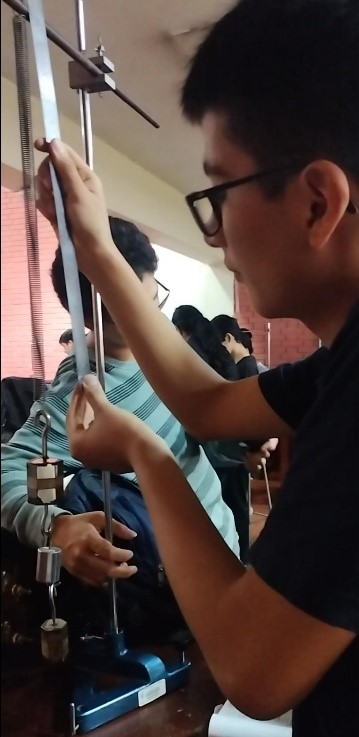
\includegraphics[width=0.6\linewidth,height=0.6\linewidth]{resources/proc1.jpg}
            \label{fig:proc1}
        \end{subfigure} &
        \begin{subfigure}{0.5\linewidth}
            \centering
            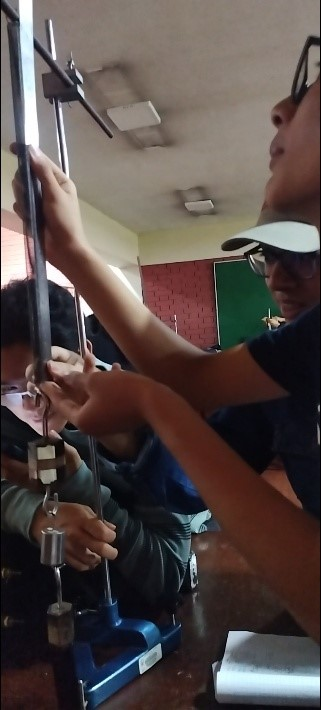
\includegraphics[width=0.6\linewidth,height=0.6\linewidth]{resources/proc2.jpg}
            \label{fig:proc2}
        \end{subfigure}\\
        \begin{subfigure}{0.5\linewidth}
            \centering
            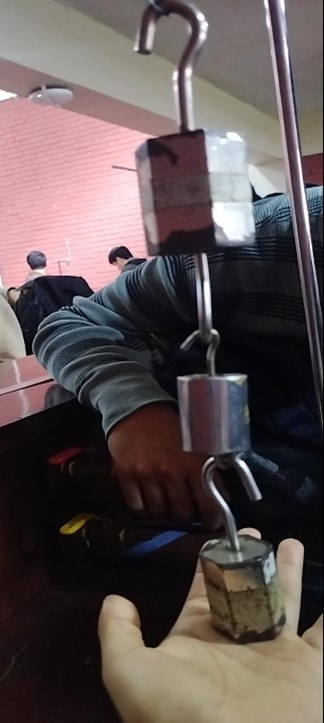
\includegraphics[width=0.6\linewidth,height=0.6\linewidth]{resources/proc3.jpg}
            \label{fig:proc3}
        \end{subfigure}&
        \begin{subfigure}{0.5\linewidth}
            \centering
            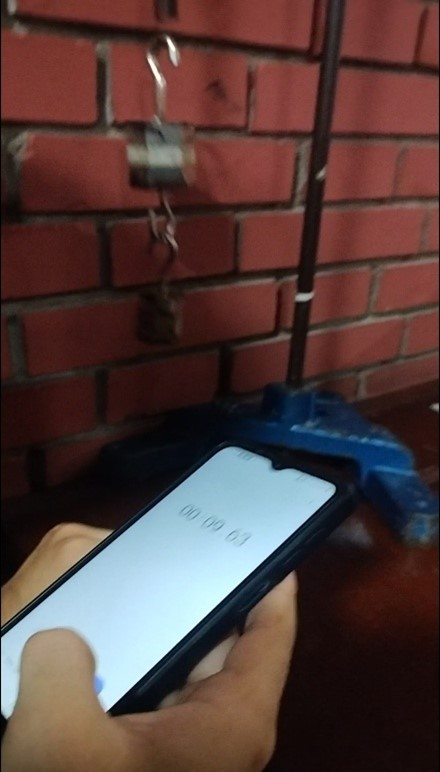
\includegraphics[width=0.6\linewidth,height=0.6\linewidth]{resources/proc4.jpg}
            \label{fig:proc4}
        \end{subfigure}\\
    \end{tabular}
    \caption{Fotografías tomadas durante la realización del procedimiento experimental.}
    \label{fig:proc_figs}
\end{figure}
\end{document}